

\documentclass[fleqn, 12pt]{article}
\usepackage[T1]{fontenc}
\usepackage{tocloft}
\usepackage[margin=1.1in]{geometry} 
\usepackage{amsmath,amsthm,amssymb,amsfonts, fancyhdr, color, comment, graphicx, environ}
\usepackage{xcolor}
\usepackage{mdframed}
\usepackage[shortlabels]{enumitem}
\usepackage{indentfirst}
\usepackage{hyperref}
\usepackage[serbian]{babel}
\renewcommand{\footrulewidth}{1 pt}
\hypersetup{
    colorlinks=true,
    linkcolor=blue,
    filecolor=magenta,      
    urlcolor=blue,
}


\pagestyle{fancy}



\newenvironment{problem}[2][Problem]
    { \begin{mdframed}[backgroundcolor=gray!20] \textbf{#1 #2} \\}
    {  \end{mdframed}}


\newenvironment{solution}{\textbf{Solution}}


\lhead{Bojan Veličković}
\rhead{Računarstvo i društvo} 
\chead{\textbf{}}
\lfoot{Prof. Sana Stojanović Đurđević}
\rfoot{Matematički fakultet, Beograd}

\renewcommand{\contentsname}{Sadržaj}
\begin{document}
\title{\Large Kurs: Računarstvo i društvo  \\[0.5cm]
        \bf\Large Bezbednost naših lozinki}
\author{\large Autor: Aleksa Jovanović\\ \ \\}
\date{\large Datum: \today}

\makeatletter
    \begin{titlepage}
        \begin{center}
	    {\ \\ \ \\}
        \vbox{}\vspace{5cm}
            {\@title }\\[3cm] 
            {\@author}
            {\large Predmetni profesor: \bf Prof. Sana Stojanović Đurđević\\  \ \\}
            {\@date\\}

        \end{center}
    \end{titlepage}
\makeatother

\setcounter{tocdepth}{2}
\tableofcontents

\newpage

\section{Istorija razvoja čet-botova}
\begin{text}
Ideja kreiranja mašine koja može da oponaša ljudski način govora i razmišljanja je nastala u isto vreme kada i prve mašine. Izumom računara, ovoj ideji počinje po prvi put da se posvećuje velika pažnja\cite{G1}.
\\\\
Čet-botovi su programi specijalizovani za komunikaciju sa čovekom. Kao unos očekuju rečenice u tekstualnom formatu, a kao rezultat daju odgovor na taj unos u tekstualnom formatu. Cilj je napraviti program koji može savršeno da imitira ljudski način pisanja. Tokom vremena su ovakvi programi prolazili kroz značajne evolucije. Od jednostavnijih programa koji su samo pratili niz pravila, do naprednih sistema veštačke inteligencije zasnovanih na mašinskom učenju\cite{G1}.
\\\\
Prvi eksperimenti sa čet-botovima potiču još iz pedesetih godina prošlog veka. Prvi takav značajan primer je bio ELIZA sistem, stvoren od strane Džozefa Vajzenbauma 1966. godine na MIT-u. ELIZA je koristila napredan sistem poklapanja šablona kako bi napravila iluziju razumevanja\cite{G1, G2, G3}.
\\\\
U narednom periodu je razvoj čet-botova bio ograničen tehničkim mogućnostima tog vremena. Razvoj je stagnirao sve do početka 21. veka kada je došlo do velikog napretka u sferi obrade prirodnih jezika (NLP). Tada virtuelni asistenti kreirani od strane velikih kompanija (Siri, Cortana, Google assistant) preuzimaju svu pažnju za sebe. Ovi asistenti su koristili kombinaciju napredih tehnika za obradu prirodnih jezika zajedno sa tadašnjim mogućnostima vestačke inteligencije kako bi dali najubedljiviji doživljaj za to vreme\cite{G1}.
\\\\
Danas, uz pomoć dubokog učenja (Deep learning) i velikih napredaka u sferi veštačke inteligencije, čet-botovi imaju mogućnosti prepoznavanja konteksta, tonaliteta, emocija. Mogu se čak i prilagođavati korisničkim potrebama u stvarnom vremenu. Predstavnici ovog novog talasa razvoja su ponovo kreirani od strane velikih kompanija (ChatGPT, Bard..). Prvi koji je probio sve prethodno postavljene granice je bio bot ChatGPT, od kompanije OpenAI, koji je pokrenuo novo interesovanje za veštačku inteligenciju i velike jezičke modele (LLM) kod mnogih programera\cite{G1}.
\end{text}
\newpage
\section{Tehnologija iza ChatGPT bota}
\begin{text}
Model koji koristi ChatGPT bot je u stanju da razume svako postavljeno pitanje i za njega generiše odgovor. Ovaj proces se dešava u više koraka.
\end{text}
\begin{enumerate}
\item Ulazna reprezentacija: Korisnik postavlja pitanje ili izjavu koju ChatGPT koristi kao ulazni signal. Ovaj ulaz se zatim prezentuje u obliku niza reči ili tokena, koji se zatim obrađuju i analiziraju\cite{G4}.
\item Obrada teksta: ChatGPT koristi napredne tehnike obrade prirodnog jezika (NLP) kako bi obradio ulazni tekst. Ovo uključuje segmentaciju teksta na tokene, lematizaciju reči, identifikaciju entiteta, analizu sentimenta i druge lingvističke analize\cite{G4}.
\item Generisanje odgovora: Nakon što je ulaz obrađen, ChatGPT koristi svoju unapred treniranu neuronsku mrežu da generiše odgovor. Neuronska mreža se sastoji od više slojeva koji obrađuju ulazne podatke i generišu odgovarajući izlaz u obliku teksta. ChatGPT bira sledeću reč u rečenici na osnovu verovatnoće njenog pojavljivanja. Ovakav sistem je sposoban da razume kontekst, tonalitet i emociju iza nekog teksta\cite{G4}.
\item Post-procesiranje: Generisani odgovor se može dodatno obrađivati kako bi se poboljšala gramatika, stil i razumljivost teksta. Ovo može uključivati korekciju pravopisa, dodavanje interpunkcije i druge korake post-procesiranja\cite{G4}.
\item Prikazivanje odgovora: Konačni odgovor se prikazuje korisniku, koji može zatim proceniti odgovor i eventualno postaviti dodatna pitanja ili izjave, što pokreće novi ciklus generisanja odgovora od strane ChatGPT-a\cite{G4}.
\end{enumerate}

\begin{figure}[h!]
    \centering
    
\includegraphics[width=0.8\textwidth]{ChatGPT-Logo.png}
    \caption{ChatGPT logo}
\end{figure}

\newpage
\section{Prednosti ChatGPT bota}
ChatGPT je napredan i besplatan alat koji je korisnicima dostupan u bilo koje vreme. Neke od njegovih prednosti su:
\begin{enumerate}
  \item Povećana pristupačnost informacijama
  \item Mogućnost korišćenja ChatGPT-a kao ličnog asistenta
  \item Mogućnost korišćenja ChatGPT-a kao pomoćnika pri učenju
  \item Prevod i provera teksta
\end{enumerate}

    \subsection{Povećana pristupačnost informacijama}
        \begin{text}
            Kreiranje interneta pokrenulo je razvoj informacione ere, a ChatGPT je samo idući korak u tom razvoju. ChatGPT može na bilo koje pitanje dati odgovor u kratkom periodu. Pre puštanja ChatGPT-a u rad (2018) alternativa ovome je bila da vršimo google pretragu i sami istražujemo to što nas zanima, a pre popularizacije interneta (1990-2000) je alternativa bila da čitamo dostupnu literaturu dok ne nađemo informaciju koju želimo. Danas možemo samo postaviti pitanje ChatGPT-u, a on nam na to pitanje odgovara za par sekundi. Ukoliko nismo zadovoljni odgovorom, moguće je postavljati dodatna potpitanja u cilju dobijanja željenog odgovora.
        \end{text}

    \subsection{Mogućnost korišćenja ChatGPT-a kao ličnog asistenta}
        \begin{text}
            ChatGPT je sposoban da samostalno smišlja odgovore na tekst koji mu prosledimo kao unos tako da imaju isti tonalitet kao taj tekst. Ovo se može iskoristiti tako što mu možemo dati zadatak da odgovara na naše poslovne mejlove. Moguće je, takođe, koristiti ga za generisanje plana dnevnih aktivnosti ili spiska potrebnih namirnica. Ovo su sve mogućnosti koje ChatGPT sam po sebi pruža, ali korišćenje ovakvog alata u sklopu nekog drugog programa drastično povećava njegove sposobnosti.\\
            Uzmimo u razmatranje prostu aplikaciju za praćenje dnevnog unosa kalorija. Ovakvu aplikaciju bi bilo moguće značajno unaprediti dodatkom ChatGPT-a, kako bi mogla da daje predloge za obroke, pa čak i da nudi recepte za pravljenje nepoznatih jela od namirnica koje su korisniku dozvoljenje. Pored toga, ChatGPT bi mogao da primeti da li nešto nedostaje u dijeti korisnika i da mu daje predloge obroka u skladu sa tim. Ovakav dodatak bi jednostavnu aplikaciju transformisao u nešto nalik ličnom nutricionisti.
        \end{text}
\newpage        
    \subsection{Mogućnost korišćenja ChatGPT-a kao pomoćnika pri učenju}
        \begin{text}
            ChatGPT je moguće koristiti kao pomoć pri učenju na nebrojano načina. Najočigledniji bi bio postavljanje pitanja ChatGPT-u svaki put kada u tekstu pročitamo nešto što nam nije potpuno jasno. Odgovori teže da drže određenu formu, tako da je, uz malo navikavanja, odmah jasno u kom delu odgovora se nalazi baš ono što nas zanima. Ukoliko, ipak, opet ne razumemo odgovor koji nam je ChatGPT dao, moguće je postavljanje potpitanja u vezi sa tim odgovorom ili zatražiti mu da ga uprosti\cite{G7}.
        \end{text}
    \subsection{Prevod i provera teksta}
        \begin{text}
            Ovaj alat je prvobitno i namenjen za prepoznavanje i obradu teksta,  tako da ovaj posao ChatGPT-u nije nimalo nepoznat. Nalaženje grešaka u tekstu je lak posao, izvršava se neprimetno i ispisuje se novi tekst bez prethodnih propusta. Moguće je prosleđivanje teksta sa zahtevom da se promeni tonalitet, ovaj posao je takođe trivijalan.
            \\
            Što se tiče prevođenja teksta, ChatGPT je sposoban da komunicira na bilo kom jeziku, tako da je prirodno da može i da prevodi prosleđeni tekst sa jednog jezika na drugi.
        \end{text}
\newpage
\section{Mane ChatGPT bota}
Uz veliki broj prednosti ovakvog alata, dolazi i veliki broj mana. Što više stvari alat omogućava, veće su sanše da će neko to iskoristiti za neke neetičke ciljeve. Zloupotreba može biti izazvana željom da se učini nesto neispravno, a može se desiti i usled nepoznavanja ispravnog načina upotrebe. Neke od mana ovakvog alata su:
\begin{enumerate}
  \item Širenje lažnih i netačnih informacija
  \item Zamena radnika mašinama
  \item Povećana zavisnost od tehnologije
  \item Identifikacija AI generisanog sadržaja i prava upotrebe
  \item Loš uticaj ChatGPT bota na obrazovni sistem
\end{enumerate}

    \subsection{Širenje lažnih i netačnih informacija}
        \begin{text}
            Uz pomoć brzine kojom ChatGPT generiše sadržaj, vrlo je moguće za jako kratko vreme napisati mnogo različitih, prividno ispravnih vesti, koje su ustvari potpuno lažne\cite{G8}.
            \\
            Slična stvar kao sa alatima koji generišu video sadržaj, koji su već u više navrata stvarali paniku pomoću širenja lažnih vesti\cite{G8}.
            \\
            Kao posledica razvoja ovakvih tehnologija nastala je mogućnost da su upravo one korišćene za pisanje članaka ili tekstova na internetu. Takvi članci neretko sadrže lažne ili neproverene informacije, obzirom da mašina ne može biti upućena u određene teme koliko neko ko se tim temama bavi. Čak i pre razvoja veštačke inteligencije i njene dostupnosti za širu javnost, informacije sa interneta je trebalo čitati uz određenu dozu rezerve, međutim, sada je to preraslo u još veći problem i lažnih vesti ima više nego ikada pre\cite{G8}.
            \\
            Sa obzirom da ChatGpt garantuje da će uvek dati odgovor, ali ne garantuje da će taj odgovor uvek biti tačan, nije čudno da se ovakve stvari dešavaju. Do ovog problema se ređe dolazi kada je reč o popularnim temama na internetu, ali postaju češće ako diskutujemo o nekoj manje popularnoj temi. Ovo je direktno povezano sa količinom sadržaja korišćenog za treniranje ChatGPT modela. Ako je količina sadržaja o nekoj temi veća, model ima odakle da se informiše. Ako se određeni sadržaj ponavlja na više mesta, postoji velika verovatnoća da je ispravan, tako da ChatGPT onda ne može napraviti grešku. Sa druge strane, ako je sadržaj na traženu temu redak, ChatGPT nema način da zaključi sta je ispravno, pa se tokom generisanja neretko provuku netacne informacije\cite{G8}.
        \end{text}
\newpage
    \subsection{Zamena radnika mašinama}
        \begin{text}
            Kao što je slučaj sa skoro svakim tehnološkim napretkom, postoje velike mogućnosti zamene radnika na određenim poslovima mašinama. ChatGPT se naročito istakao svojim poznavanjem programiranja na osnovnom, pa i malo višem nivou. Danas, jedan programer junior, uz pomoć ChatGPT-a potencijalno može znatno brže da uradi neki posao nego što je to bilo moguće pre. Naravno, ovakav alat nikako ne može u potpunosti zameniti junior programere, ali može stvoriti takve uslove da ih bude potrebno manje. Takođe, treba uzeti u obzir da će ovaj alat da nastavi da se razvija i da će vremenom postajati sve bolji. U nekom trenutku će biti moguće napraviti ChatGPT koji je specijalizovan za programiranje, pa će tada potpuna zamena juniora možda biti ideja bliža realnosti nego sto je to slučaj sada\cite{G6}.
        \end{text}

    \subsection{Povećana zavisnost od tehnologije}
        \begin{text}
            Ljudska priroda je da uvek težimo ka najlakšem rešenju problema. Baš ta priroda može dovesti do toga da počnemo previše da se oslanjamo na ovakve alate, a manje na naše razmišljanje. Posledica ovoga je da se od malih nogu odričemo sposobnosti kritičkog rasuđivanja i razmišljanja, zarad lakših rešenja problema pomoću ChatGPT-a.
            \\\\
            Slično ovome, dokazano je da oslanjanje na GPS aplikacije, poput Google maps, negativno utiče na razvoj sposobnosti snalaženja u prostoru. U jednom istraživanju je pokazano da ispitanici koji su se oslanjali na GPS aplikacije mnogo slabije pamte puteve i teže se snalaze u svom gradu od ispitanika koji se snalaze pomocu papirne mape grada\cite{G5}.
            
        \end{text}
\newpage
    \subsection{Identifikacija AI generisanog sadržaja i prava upotrebe}
        \begin{text}
            Slično širenju lažnih vesti, jedan od većih problema je, takođe, teško prepoznavanje kada je neki sadržaj pisao robot, a kada čovek. ChatGPT je toliko napredan alat, da u većini slucajeva nije moguće primetiti razliku.
            \\
            Recimo da dve osobe komuniciraju putem e-pošte. Ako jedna od te dve osobe pusti ChatGPT da u potpunosti odgovara umesto nje bez javljanja osobi sa druge strane, da li bi ta druga osoba mogla da zaključi da ne priča sa ljudskim bićem? Koliko razmenjenih mejlova bi bilo potrebno pre nego sto se to desi? Da li bi se uopšte desilo?
            \\\\
            Dodatni problem predstavlja da je ChatGPT treniran na velikoj količini ljudski generisanog sadržaja koji se može naći na internetu. Zbog ove činjenice, generisan sadržaj ChatGPT-a bi mogao da se smatra krađom intelektualne svojine. Sa jedne strane, čitanje već postojećeg sadržaja kako bi stekli razumevanje i pisali svoje radove je stvar koju ljudi redovno rade. Da li stvarno postoji razlika ako isto to radi mašina?
            \\
            Glavna razlika između ljudi i ChatGPT-a se nalazi u razumevanju. ChatGPT nema mogućnost razumevanja sadržaja. Kao čet-bot, on samo pokušava da generiše najbolji mogući odgovor po njegovom internom spisku kriterijuma. Model ne razume reči koje piše, niti poznaje smisao koji stoji iza njih. Zbog toga, kada ChatGPT generiše sadržaj, to je više nalik uzimanju tuđeg sadržaja i preformulisanje nego razmevanje tog sadržaja i kreiranje svog.
        \end{text}

    \subsection{Loš uticaj ChatGPT bota na obrazovni sistem}
        \begin{text}
            Postoji nekoliko aspekata upotrebe ChatGPT-a koji mogu biti problematični u kontekstu obrazovanja\cite{G7}.
            \\\\
            Prvo, ChatGPT može doprineti smanjenju kritičkog razmišljanja i samostalnog istraživanja kod učenika. Kada se učenici prečesto oslanjaju na ChatGPT za odgovore, postoji opasnost da će izgubiti navedene veštine\cite{G7}.
            \\\\
            Drugo, ChatGPT može pružiti neproverene ili nepouzdane informacije. Budući da ChatGPT generiše odgovore na osnovu ogromnog skupa podataka na internetu, moguće je da će generisati odgovore koji su netačni ili zastareli. Ovo može dovesti do širenja dezinformacija i pogrešnih shvatanja među učenicima\cite{G7}.
            \\\\
            Treće, ChatGPT može narušiti interpersonalnu komunikaciju i razvoj socijalnih veština kod učenika. Korišćenje ChatGPT-a kao zamene za interakciju s nastavnicima i kolegama može smanjiti prilike za razvoj veština komunikacije, empatije i saradnje\cite{G7}.
        \end{text}
        
\newpage
\section{Budućnost razvoja ChatGPT sistema}
\begin{text}
Sistemi poput ChatGPT-a su tek krenuli sa svojim razvojem, a čak i u svojim prvim iteracijama su našli široku primenu, dok interesovanje za njih samo raste.
\\
Što se tiče daljeg razvoja, postoje beskrajne mogućnosti. Planovi za treniranje modela koji koristi ChatGPT da tacnije i brže prepoznaje kontekst korisničkih poruka, već bivaju implementirani, 
kao i adaptivno učenje na osnovu prethodnih konverzacija i kreiranje potpuno novih modela, nalik modelu koji koristi ChatGPT, koji bi bili specijalizovani za konkretne oblasti (programiranje, zdravstvo, školovanje, finansije..)\cite{G9}.
\\\\
Moguće je i kombinovati ovakve modele sa modelima drugih namena. U skorašnjoj konferenciji za novinare kompanije OpenAI, predstavljen je robot koji u sebi ima niz modela koji mu omogućavaju da prima ulaz u obliku izgovorenih rečenica od strane korisnika, taj unos zatim prevodi u tekstualni format i prosleđuje ga ChatGPT modelu koji može u stvarnom vremenu dati odgovore na zadata pitanja i da ih prosledi sledećem modelu koji ih iz tekstualnog formata prevodi u audio. Drugim rečima ovo je robot koji uspešnim korišćenjem niza modela može da komunicira sa korisnikom u realnom vremenu\cite{G10}.
\\
Pored toga, ovaj robot je bio opremljen modernim kamerama i senzorima, kako bi mogao da prepoznaje svoje okruženje i odgovara na pitanja tipa "Šta se nalazi ispred tebe". Takođe, uz pomoć modernih motora ugrađenih u svaki zglob ovog robota, on ima mogućnost izvršavanja prostih poslova. Ovaj robot je dobio naziv Figure01\cite{G10}.
\end{text}

\begin{figure}[h]
    \centering
    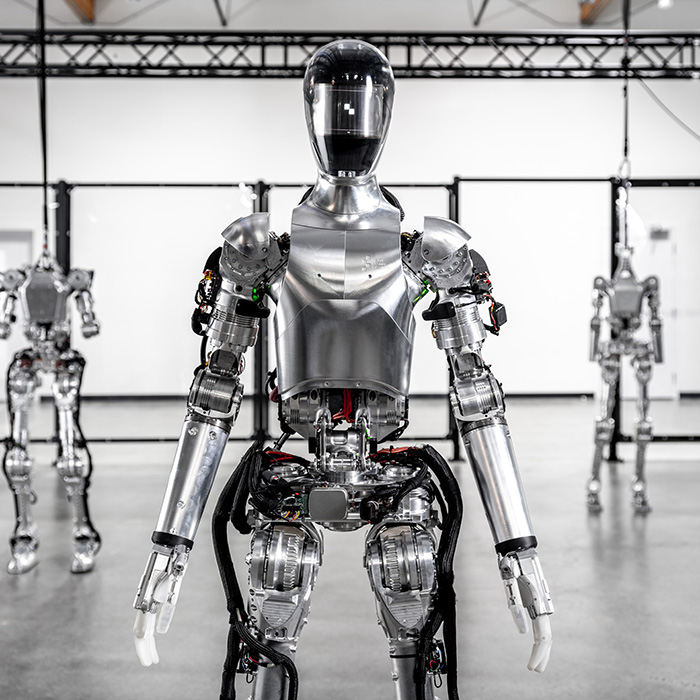
\includegraphics[width=0.5\textwidth]{Figure.jpg}
    \caption{Figure01 kompanije Figure}
\end{figure}

\newpage
\section{Zaključak}
\begin{text}
Iako veštačka inteligencija dolazi sa velikim brojem prednosti i  rešenja za svakodnevne probleme, ipak uz to ima i svojih mana. Svaki alat je moguće iskoristiti u neetičke svrhe, namerno ili slučajno. Tako da, kao i za svaki alat, tako i za veštačku inteligenciju važi da je bitno koristiti je sa oprezom, kao i informisati se o najboljem načinu korišćenja. Dodatno, bitno je obratiti pažnju na problem krađe intelektualne svojine. Povećana pristupačnost informacijama nije loša stvar, ali nekada je jako bitno znati odakle je ChatGPT dobio informacije koje nam daje. Trenutno je nemoguće to saznati, ali sigurno ne bi bilo loše da ChatGPT u svojim odgovorima sam to napiše kao spisak referenci. Takođe, ChatGPT treba da se koristi kao dopuna tokom informisanja o određenoj temi i na njega se ne treba u potpunosti oslanjati.
\\
Za kraj, ChatGPT ima neosporivu vrednost kao alat koji je moguće koristiti u različite svrhe i uprkos svim svojim nedostacima, ostaje koristan alat sa neverovatnim potencijalom, pogotovo kada se koristi sa razumevanjem njegovih ograničenja.
\end{text}
{
\raggedright
\renewcommand{\refname}{Reference}
\begin{thebibliography}{9}
    \bibitem{G1} The History Of Chatbots – From ELIZA to ChatGPT (2022), Članak autora Ina, dostupan on-line na \href{https://onlim.com/en/the-history-of-chatbots/}{onlim.com}
    
    \bibitem{G2} Norvig, Peter (1992), ELIZA: Paradigms of Artificial Intelligence Programming
    
    \bibitem{G3} Weizenbaum, Joseph (1976), Computer power and human reason: from judgment to calculation
    
    \bibitem{G4} How does ChatGPT actually work?(2023), Članak autora David Gewirtz, dostupan on-line na \href{https://www.zdnet.com/article/how-does-chatgpt-work/}{zdnet.com}
    
    \bibitem{G5} Google Maps Is Melting Your Brain (2020), Članak autora Angela Lashbrook, dostupan on-line na \href{https://debugger.medium.com/google-maps-is-melting-your-brain-a9b34adc0936}{Medium}
    
    \bibitem{G6} Can we replace junior developers with ChatGPT? (2023), Članak autora Alex Hyett, dostupan on-line na  \href{https://dev.to/alexhyettdev/can-we-replace-junior-developers-with-chatgpt-343h }{dev.to}
    
    \bibitem{G7} The influence of ChatGPT and AI Tools on the Academic Performance (2023), Istraživački rad autora Togzhan Nurtayeva, Mohammed Salim, Savriddin Khalilov i Taha Basheer, dostupan on-line na \href{https://www.researchgate.net/publication/371405528_The_influence_of_ChatGPT_and_AI_Tools_on_the_Academic_Performance}{researchgate.com}
        
    \bibitem{G8} Disinformation Researchers Raise Alarms About A.I. Chatbots (2023), Članak autora Tiffany Hsu i Stuart A. Thompson u \href{https://www.nytimes.com/2023/02/08/technology/ai-chatbots-disinformation.html}{NewYorkTimes}
        
    \bibitem{G9} The future of ChatGPT: predictions and opportunities (2023), Članak u AIContentify časopisu, dostupan on-line na \href{https://aicontentfy.com/en/blog/future-of-chatgpt-predictions-and-opportunities}{aicontentify.com}
    
    \bibitem{G10} ChatGPT Has a Body Now: What Is Figure 01 and How Does it Work? (2024), Članak autora Aaron Drapkin, dostupan on-line na \href{https://tech.co/news/what-is-figure-01-chatgpt}{tech.to}
\end{thebibliography}
}
\end{document}